\subsection{Results for Speed}
%\label{subsec:speed_results}
%\vspace{10pt}

Figure~\ref{fig:var_speed_RMSE} represents the $p$-values for the Wilcoxon signed-rank test on RMSE values across $k$-fold validation datasets for the speed in the $k$-fold testing datasets using different RNN models, and forecasting times. Darker colors in grayscale represent a higher $p$-value in a range from $0$ to $1$. The values on the secondary diagonal are all equal to $1$ and black because models equal themselves.

\begin{figure}[!ht]
	\centering
	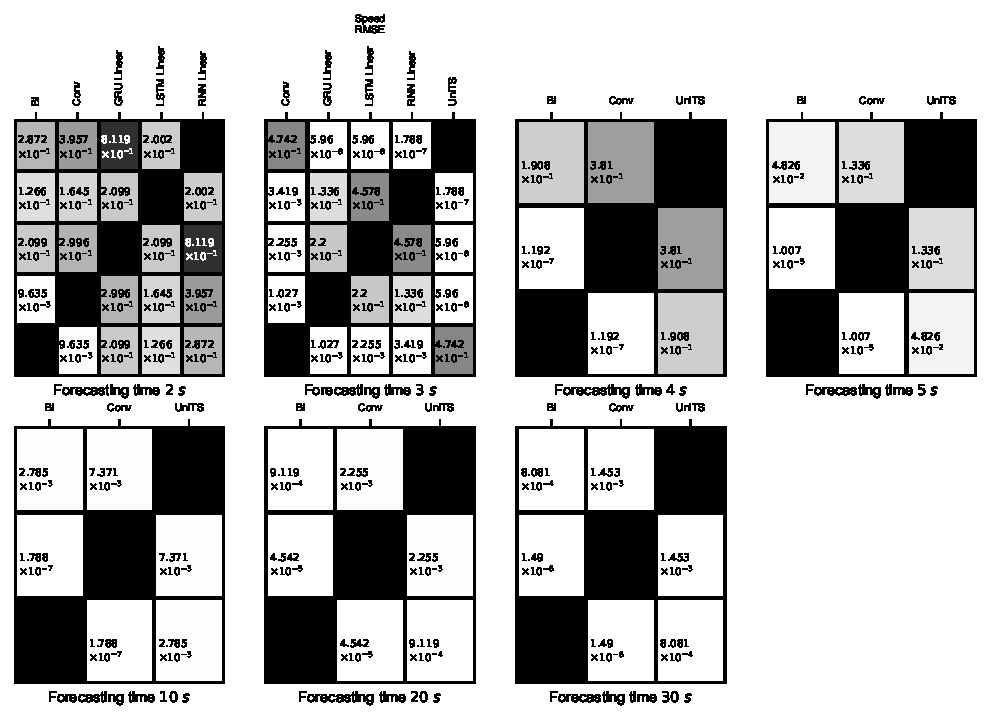
\includegraphics[width = 0.99 \linewidth]{var_speed_RMSE.pdf}
	\caption{The $p$-values for the Wilcoxon signed-rank test on RMSE values across $k$-fold validation datasets for the speed in the $k$-fold testing datasets using different RNN models, and forecasting times. Darker colors in grayscale represent a higher $p$-value in a range from $0$ to $1$. The values on the secondary diagonal are all equal to $1$ and black because models equal themselves.}
	\label{fig:var_speed_RMSE}
\end{figure}

The average RMSE in $km/h$, with standard deviation in brackets, across $k$-fold validation datasets for the speed estimated on the $k$-fold testing datasets by different RNN models, and forecasting times is listed in Table~\ref{tab:wilcoxon_speed_RMSE}.

\begin{table}[!ht]
	\centering
	\resizebox{\linewidth}{!}{
		\begin{tabular}{|c|c|c|c|c|c|c|c|}
			\hline
			Model & $2$ $s$ & $3$ $s$ & $4$ $s$ & $5$ $s$ & $10$ $s$ & $20$ $s$ & $30$ $s$ \\ \hline
			\multirow{2}{*}{Bi} & $4.179$ & $5.259$ & $6.199$ & $6.994$ & $9.488$ & $11.359$ & $12.115$ \\
			 & ($0.303$) & ($0.37$) & ($0.43$) & ($0.482$) & ($0.63$) & ($0.689$) & ($0.744$) \\ \hline
			\multirow{2}{*}{Conv} & $4.161$ & $\mathbf{5.199}$ & $6.12$ & $6.931$ & $9.409$ & $11.29$ & $12.022$ \\
			 & ($0.296$) & \textbf{(}$\mathbf{0.374}$\textbf{)} & ($0.431$) & ($0.479$) & ($0.64$) & ($0.698$) & ($0.713$) \\ \hline
			\multirow{2}{*}{GRU Linear} & $4.059$ & $5.654$ & $6.986$ & $7.896$ & $10.444$ & $11.469$ & $11.854$ \\
			 & ($0.283$) & ($0.481$) & ($0.534$) & ($0.589$) & ($0.812$) & ($0.798$) & ($0.755$) \\ \hline
			\multirow{2}{*}{LSTM Linear} & $\mathbf{4.026}$ & $5.609$ & $6.866$ & $7.878$ & $10.372$ & $11.435$ & $11.901$ \\
			 & \textbf{(}$\mathbf{0.301}$\textbf{)} & ($0.447$) & ($0.528$) & ($0.593$) & ($0.707$) & ($0.753$) & ($0.76$) \\ \hline
			\multirow{2}{*}{RNN Linear} & $4.053$ & $5.589$ & $6.859$ & $7.755$ & $10.232$ & $11.323$ & $11.807$ \\
			 & ($0.344$) & ($0.472$) & ($0.533$) & ($0.625$) & ($0.785$) & ($0.803$) & ($0.696$) \\ \hline
			\multirow{2}{*}{UniTS} & $4.353$ & $5.246$ & $\mathbf{6.022}$ & $\mathbf{6.691}$ & $\mathbf{8.861}$ & $\mathbf{10.555}$ & $\mathbf{11.262}$ \\
			 & ($0.296$) & ($0.369$) & \textbf{(}$\mathbf{0.424}$\textbf{)} & \textbf{(}$\mathbf{0.473}$\textbf{)} & \textbf{(}$\mathbf{0.639}$\textbf{)} & \textbf{(}$\mathbf{0.772}$\textbf{)} & \textbf{(}$\mathbf{0.754}$\textbf{)} \\ \hline
		\end{tabular}
	}
	\caption{The average RMSE in $km/h$, with standard deviation in brackets, across $k$-fold validation datasets for the speed estimated on the $k$-fold testing datasets by different RNN models, and forecasting times.}
	\label{tab:wilcoxon_speed_RMSE}
\end{table}

The Conv model achieved the lowest RMSE for speed, and a forecasting time of $3$ $s$ with an average value and standard deviation (in brackets) that equals $5.2$ $km/h$ ($0.37$ $km/h$).

The Conv model does not have a statistically significantly different RMSE than the GRU Linear, LSTM Linear, RNN Linear, and UniTS models for speed using a forecasting time of $3$ $s$, with $p$-values equaling $1.027 \times 10^{-3}$, $2.255 \times 10^{-3}$, $3.419 \times 10^{-3}$, and $4.742 \times 10^{-1}$.

\markertable{tab:\label{tab:RMSE:speed:p:3}}

The LSTM Linear model achieved the lowest RMSE for speed, and a forecasting time of $2$ $s$ with an average value and standard deviation (in brackets) that equals $4.03$ $km/h$ ($0.3$ $km/h$).

The LSTM Linear model does not have a statistically significantly different RMSE than the Bi, Conv, GRU Linear, and RNN Linear models for speed using a forecasting time of $2$ $s$, with $p$-values equaling $1.266 \times 10^{-1}$, $1.645 \times 10^{-1}$, $2.099 \times 10^{-1}$, and $2.002 \times 10^{-1}$.

\markertable{tab:\label{tab:RMSE:speed:p:2}}

The UniTS model achieved the lowest RMSE for speed, and a forecasting time of $4$, $5$, $10$, $20$, and $30$ $s$ with average values and standard deviation (in brackets) that equal $6.02$ $km/h$ ($0.42$ $km/h$), $6.69$ $km/h$ ($0.47$ $km/h$), $8.86$ $km/h$ ($0.64$ $km/h$), $10.55$ $km/h$ ($0.77$ $km/h$), and $11.26$ $km/h$ ($0.75$ $km/h$) respectively.

The UniTS model does not have a statistically significantly different RMSE than the Bi, and Conv models for speed using a forecasting time of $4$ $s$, with $p$-values equaling $1.908 \times 10^{-1}$, and $3.81 \times 10^{-1}$.

\markertable{tab:\label{tab:RMSE:speed:p:4}}

The UniTS model does not have a statistically significantly different RMSE than the Bi, and Conv models for speed using a forecasting time of $5$ $s$, with $p$-values equaling $4.826 \times 10^{-2}$, and $1.336 \times 10^{-1}$.

\markertable{tab:\label{tab:RMSE:speed:p:5}}

The UniTS model does not have a statistically significantly different RMSE than the Bi, and Conv models for speed using a forecasting time of $10$ $s$, with $p$-values equaling $2.785 \times 10^{-3}$, and $7.371 \times 10^{-3}$.

\markertable{tab:\label{tab:RMSE:speed:p:10}}

The UniTS model does not have a statistically significantly different RMSE than the Bi, and Conv models for speed using a forecasting time of $20$ $s$, with $p$-values equaling $9.119 \times 10^{-4}$, and $2.255 \times 10^{-3}$.

\markertable{tab:\label{tab:RMSE:speed:p:20}}

The UniTS model does not have a statistically significantly different RMSE than the Bi, and Conv models for speed using a forecasting time of $30$ $s$, with $p$-values equaling $8.081 \times 10^{-4}$, and $1.453 \times 10^{-3}$.

\markertable{tab:\label{tab:RMSE:speed:p:30}}

